\subsubsection{Strøm}
\paragraph{Frie elektroner i bevegelse} \mbox{} \\
Hvis et elektron slipper løs fra et atom kan det bevege seg fra et atom til et annet.
Når slike "frie elektroner" beveger seg gjennom gjennom en ledning
har vi det som kalles elektrisk strøm.
\\

Strømretningen er definert som den retningen elektronene beveger seg.
Altså fra negativ til positiv.\\
NB! Det har lenge vært vanlig å definere strømretningen motsatt fra dette.
\\
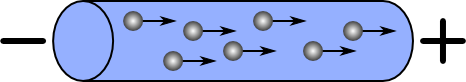
\includegraphics[scale=0.5]{./img/current}

\paragraph{Enhet} \mbox{} \\
Strøm måles etter hvor mange ladninger som passerer et punkt
i løpet av et sekund.
SI enheten for strøm er Ampere (A) \hfill $\SI{1}{\ampere} = C/s$
